% Main text of the article: the demographic-noise model.  Derivations, checks and robustness are in
% the Supplemental Material, sm.tex in this directory.  The deterministic life-cycle theory (exact
% one-firm solution, kill rule, lifetime law) is notebooks/03_life_cycles.ipynb.
% Build: latexmk -pdf paper.tex   (from this directory)
%
% Draft status (2026-10-11): rewritten around the demographic model, with the multiscaling
% mechanism as the main result.  Reference point alpha 2.5, sigma 1.70, D 0.1, C 200.  Numbers
% marked \todo{} need a computation that does not exist yet or a re-run.  Every figure in figures/
% is written by a notebook in ../notebooks/.
\documentclass[pre,twocolumn,superscriptaddress,nofootinbib]{revtex4-2}
\usepackage{amsmath,amssymb,bm}
\usepackage{graphicx}
\usepackage{xcolor}
\graphicspath{{figures/}}
\usepackage[hidelinks]{hyperref}

\newcommand{\E}{\mathbb E}
\newcommand{\Var}{\operatorname{Var}}
\newcommand{\Sb}{\bar S}
\newcommand{\todo}[1]{\textcolor{red}{[TODO: #1]}}

\begin{document}

\title{Interaction heterogeneity and the multiscaling of firm growth volatility}
\author{Ludovico Furlanetto}
\date{\today}

\begin{abstract}
The growth volatility of firms falls with their size as $\E[v^q\mid\Sb]\sim\Sb^{-\zeta_q}$ with
$\zeta_1\simeq0.2$, and the ratios $\zeta_q/\zeta_1$ fall below $q$: the shape of the volatility
distribution changes with size.  Granular models, in which a firm is a sum of independent parts,
give a volatility law of fixed shape and therefore $\zeta_q=q\zeta_1$.  We study instead an economy of
interacting firms: a generalised Lotka--Volterra model on a scale-free network, with interactions
and self-limitation measured in units of the mean firm, birth--death noise, and replacement of
exiting firms by newborns.  Heterogeneous mean-field theory gives the line above which the economy
keeps fluctuating, and an exact renewal law for a single node predicts its turnover.  In the
fluctuating phase each firm behaves as a logistic unit driven by its own field, whose amplitude
grows as the square root of its degree.  A firm's growth variance is then the sum of a fitness floor,
nearly independent of size, and a demographic part that falls with size, so $\zeta_1\simeq0.2$ is the
effective slope of a crossover from slope $-1/2$ to slope $0$.  We show that for any such two-part law
$\zeta_q=(q/2)\,b\,\langle w\rangle_q$, with $w$ the demographic share of the variance, and that the ratio
curve bends below $q$ if and only if the floor differs between firms of equal size.  On the network
the floor grows with the degree; the floor's heterogeneity alone predicts ratios $1.86$, $2.57$, $3.10$
against $1.77$, $2.35$, $2.78$ measured and $2.0$, $2.6$, $2.9$ in Compustat, while a graph with equal
degrees, where the floor stays small against the noise, gives ratios close to $q$.  The same self-limitation that produces the decline caps firm size, so the model
has no Zipf law and the decline spans two decades rather than four; without noise the product of the
exponent and the range is fixed by the self-limitation.
\end{abstract}

\maketitle

%======================================================================
\section{Introduction}
\label{sec:intro}

Large firms grow less erratically than small ones, but much more erratically than a sum of
independent parts would.  If $v$ is the volatility of a firm's growth rate and $\Sb$ its mean size
over its life, the conditional moments in Compustat scale as
\begin{equation}
\E[v^q\mid\Sb]\sim\Sb^{-\zeta_q},\qquad \zeta_q=0.20,\ 0.39,\ 0.51,\ 0.58,
\label{eq:zeta}
\end{equation}
for $q=1,\dots,4$,
over four decades of size \cite{stanley1996,amaral1997,sutton2002,moran2024}.  The ratios
$\zeta_q/\zeta_1=2.0$, $2.6$, $2.9$ lie below $q$ \cite{moran2024}.  If a firm's volatility were a
function of its size times a random factor with a size-independent law, the ratios would be exactly
$q$; the bend means that the dispersion of volatilities among firms of equal size grows with size.
Moran, Secchi and Bouchaud \cite{moran2024} (MSB) add further facts: the volatility divided by its
size-conditional mean has a universal distribution with a power-law tail of index $b\simeq4.6$,
rescaled growth rates stay fat-tailed at every size, multi-year growth is persistent, and a firm's
co-movement with the aggregate rises with its size.  Firm sizes follow Zipf's law \cite{axtell2001}.

Granular models, in which a firm is a sum of subunits with independent shocks
\cite{wyartbouchaud2003,gabaix2011}, give $\zeta_1<1/2$ when the subunit sizes are broad, but in
their scaling regime the law of the rescaled volatility does not depend on size, so
$\zeta_q=q\zeta_1$; MSB show that they also fail the universality of the volatility distribution and
the absence of Gaussianisation \cite{moran2024}.  Data that include very small firms show a steep
decline, close to slope $-1/2$, for small firms and a nearly flat relation for large ones
\cite{fontanelli2025}, which suggests a crossover rather than a single power law.

Here we ask whether interactions between firms can produce these facts.  Our starting point is the
disordered generalised Lotka--Volterra (GLV) model, whose strongly interacting phase keeps
fluctuating: species exchange the roles of rare and abundant, and each behaves as a logistic unit
driven by a coloured Gaussian field \cite{roy2020,mallmin2024,arnouxbunin2024}.  We make three
changes to adapt it to firms.  Interactions and self-limitation are measured in units of the mean
firm, so that the economy has no preferred size and grows at a rate the dynamics selects.  Firms
sit on a scale-free network, as production and competition networks do
\cite{acemoglu2012,carvalho2019}.  And the immigration that keeps species from extinction is
replaced by birth--death noise with turnover: a firm that reaches zero exits and a newborn takes its
place.  The model has five parameters: the mean $\mu$ and spread $\sigma$ of the interactions, the
degree tail $\alpha$ and mean degree $C$, and the noise $D$.

Our results are the following.
\begin{enumerate}
\item The phase diagram (Sec.~\ref{sec:phase}): heterogeneous mean-field theory gives the line
  $\sigma_c$ above which the composition of the economy keeps changing, in closed form to first
  order in the degree variance, and its shift with the noise, $\sigma_c(D)$, from an exact renewal law
  for a single node, which also predicts the turnover rate.
\item One firm is enough (Sec.~\ref{sec:onefirm}): a firm driven by its own measured field and its own
  noise reproduces the size--volatility statistics of the full economy, and the field has a
  degree-resolved Gaussian law whose amplitude grows as $\sqrt\kappa$ with the relative degree
  $\kappa$.
\item A volatility law (Sec.~\ref{sec:law}): a firm's growth variance is a fitness floor, nearly
  independent of size, plus demographic noise filtered by the firm's relaxation.  The exponent
  $\zeta_1\simeq0.2$ is the effective slope of the crossover between them.
\item The multiscaling mechanism (Sec.~\ref{sec:multiscaling}), our main result: for any law of the
  form floor plus size-dependent part, $\zeta_q=(q/2)\,b\,\langle w\rangle_q$ up to a composition term, and the ratio curve
  bends below $q$ if and only if the floor differs between firms of equal size.  On the network the
  floor grows with the degree, and its heterogeneity predicts the measured ratio curve; on a graph
  with equal degrees the ratios return close to $q$.
\item A comparison with every MSB fact (Sec.~\ref{sec:facts}) and a structural limit
  (Sec.~\ref{sec:limits}): the self-limitation that makes volatility depend on size also caps firm
  size, so the range of the decline and the exponent trade off, and the model has no Zipf law.
\end{enumerate}
Derivations, numerical checks and robustness tests are in the Supplemental Material (SM).

%======================================================================
\section{Model}
\label{sec:model}

Firm $i=1,\dots,N$ has size $x_i$ and $m=N^{-1}\sum_jx_j$ is the mean firm.  Firms sit on the nodes
of a configuration-model graph with degree law $p(k)\propto k^{-\alpha}$ and mean degree $C$.  The
sizes obey
\begin{equation}
dx_i=x_i\Big[1-\frac{x_i}{m}+\sum_jJ_{ij}\frac{x_j}{m}\Big]dt+\sqrt{D\,m\,x_i}\;dW_i ,
\label{eq:model}
\end{equation}
with independent Wiener processes $W_i$ and couplings $J_{ij}=A_{ij}(\mu/C+\sigma z_{ij}/\sqrt C)$, where $A$
is the adjacency matrix and $z_{ij}$ are independent standard Gaussians ($z_{ij}$ and $z_{ji}$
uncorrelated).  $\mu<0$ is net competition.  A firm that reaches $x_i=0$ exits, and a newborn of size
$Dm$ takes its node and its couplings: a new firm in the same niche.

Each term is the one of the standard GLV with the carrying capacity and the interaction unit set to
the mean firm, and the noise is the birth--death noise of stochastic population models
\cite{altieri2021} with unit $Dm$.  Every term is homogeneous of degree one in the sizes, so the
economy has no preferred size: $m$ grows at a rate selected by the dynamics, and a firm is large or
small only relative to the others.  The noise unit $Dm$ grows with the economy; it can be read as an
indivisible unit of business (a contract, a customer) whose size follows the mean firm.  In a
deterministic version of the model, studied in earlier work, the noise is replaced by an immigration
floor $\lambda(m-x_i)$; that version is the $D\to0$ limit of the phase diagram below, and its one-firm
theory is in a separate note.

With relative sizes $S_i=x_i/m$, Eq.~\eqref{eq:model} becomes
\begin{equation}
dS_i=S_i\big[\Phi_i(t)-S_i\big]dt+\sqrt{DS_i}\,dW_i+O(N^{-1/2}),
\label{eq:onefirm}
\end{equation}
with the field
\begin{equation}
\Phi_i(t)=1+\sum_jJ_{ij}S_j(t)-\bar f(t),\qquad \bar f=\frac{\dot m}{m},
\label{eq:field}
\end{equation}
and $\bar f=N^{-1}\sum_iS_i(1-S_i+\sum_jJ_{ij}S_j)$ the growth rate of the mean firm.  The $O(N^{-1/2})$
term keeps $\sum_iS_i=N$.  Exit is at $S_i=0$ and entry at $S_i=D$.  Equation~\eqref{eq:onefirm} is a
logistic equation with a moving carrying capacity: a firm whose field stays at $\Phi$ relaxes to the
plateau $x_i=m\Phi$ at rate $\Phi$, and a firm with $\Phi<0$ shrinks to exit.  For $C\to\infty$ and a
growth rate that self-averages, a rescaling of size and time maps the relative sizes onto the
standard GLV with demographic noise \cite{altieri2021} and renormalised parameters (SM, Sec.~S1); on the
complete graph and with an immigration floor in place of the noise this is the chaotic-turnover model
of Refs.~\cite{bunin2017,mallmin2024}.  The normalisation adds
the growth rate as an output and observables measured relative to the mean firm, as in firm data.

\paragraph{Numerics and protocol.}  We integrate Eq.~\eqref{eq:model} in relative form by
Euler--Maruyama with step $0.01$, discard $t<100$ and record sizes every $\Delta t=0.5$, which we take as
one year (SM, Sec.~S6), over a window of $480$.  Following MSB we use an unbalanced panel: a \emph{life}
runs from a birth to the next exit at the same node, lives cut by the window are kept, and a life's
volatility is $v=\sqrt{\pi/2}$ times the mean absolute deviation of its yearly growth rates
$g=\Delta\ln S$ around their mean.  $\Sb$ is the life's mean relative size, and lives need at least
$n_{\min}$ growth rates.  Exponents are least-squares slopes of $\ln\E[v^q\mid\Sb]$ against $\ln\Sb$ over
$25$ equal-count bins, all bins included.  The reference point is $\alpha=2.5$, $\sigma=1.70$, $D=0.1$,
$C=200$, $\mu=-1.76$.  The facts of Sec.~\ref{sec:facts} come from eight economies with $N=32000$, one of
which, in a collective burst, is excluded (SM, Sec.~S5); the theory tests use two economies with
$N=16000$.

%======================================================================
\section{Phase diagram}
\label{sec:phase}

\paragraph{Deterministic limit.}  For $C\to\infty$ the field on a firm of relative degree
$\kappa=k/C$ is Gaussian.  Heterogeneous dynamical mean-field theory (HDMFT) replaces the network by
one process per degree class, closed by averages over neighbours, which are drawn in proportion to
their degree \cite{aguirrelopez,patil2026}:
\begin{equation}
\Phi(t)=1-\bar f(t)+\mu\kappa\bar B+\sigma\sqrt\kappa\,\xi(t),
\label{eq:hdmft}
\end{equation}
with $\bar B$ the degree-weighted mean size and $\xi$ a Gaussian process whose correlation is the
degree-weighted correlation of sizes.  Without noise and with a vanishing floor, the stationary sizes
are clipped Gaussians, and the unique fixed point of the composition loses stability when the Perron
root of $\sigma^2\varphi_pK_{pr}$ reaches one, with $\varphi_p$ the fraction of surviving firms in class $p$
and $K_{pr}$ the class kernel.  On an uncorrelated graph the stability operator has rank one, and to
first order in the degree variance
\begin{equation}
\sigma_c\simeq\sqrt2\Big[1-\frac{\Var\kappa}{2}\Big(1-\frac{\mu^2}{2\pi}\Big)\Big]
\label{eq:sigmac}
\end{equation}
(SM, Sec.~S2).  Degree heterogeneity lowers the threshold because hubs feel a field of amplitude
$\propto\sqrt\kappa$; competition raises it because it removes the noisiest firms.  The line on which the
economy stops growing hardly depends on the network: its shift is at most a third of that of
$\sigma_c$.

\paragraph{Renewal law.}  With noise and turnover, a node whose field is constant is a renewal
process: its successive lives are independent and identically distributed.  Equation~\eqref{eq:onefirm}
at constant $\Phi=h$ is a one-dimensional diffusion with scale density
$s'(y)=\exp[-(2/D)(hy-y^2/2)]$ and speed density $m(y)=2/(Dy\,s'(y))$, and by the renewal--reward theorem
the fraction of time the node spends at size $x$ is
\begin{gather}
p(x\mid h)=\frac{s(\min(x,D))\,m(x)}{T(D)},\nonumber\\
T(D)=\int_0^\infty s(\min(x,D))\,m(x)\,dx,
\label{eq:renewal}
\end{gather}
with turnover rate $1/T(D)$.  The law has two parts: a Gaussian plateau of variance $D/2$ around $h$,
and below $D$ a nearly flat density of newborns drifting to exit.  Establishment probabilities and
exit times follow from the same quadratures and agree with direct simulation to $1.5\%$ (SM,
Sec.~S3).

\paragraph{Instability line with noise.}  Replacing the clipped Gaussian by the renewal law in the
static self-consistency gives the mean sizes $\langle S\rangle_h$ and the susceptibility
$\chi=\partial\langle S\rangle_h/\partial h$; the static state is stable while the Perron root of
$\sigma^2{\rm diag}(\E\chi^2)K$ is below one.  Noise smooths $\chi$ and raises the line almost linearly with
$D$ (SM, Fig.~S1): from $1.460$ to $1.577$ at $\alpha=2.5$ and from $1.399$ to $1.551$ at
$\alpha=6$ between $D=0.003$ and $0.3$; as $D\to0$ it tends to the deterministic line ($1.399$ against
$1.400$ at $\alpha=6$, and $\sqrt2$ on the complete graph).  The same theory predicts the turnover rate
to $0.5\%$ below $\sigma_c$ and to $1.5\%$ above it, where it is no longer controlled ($\alpha=6$; SM,
Sec.~S3).  Turnover is set by
the nodes with $h<0$, where a newborn's life does not depend on $D$, and is nearly independent of the
noise.  Figure~\ref{fig:phase} shows the phase diagram in the plane of the mean interaction and the
disorder.  On the reference graph competition raises $\sigma_c$ strongly, from $0.83$ at $\mu=0$ to $1.68$ at
$\mu=-2.5$, because it removes the hubs, which carry the strongest fields; on the complete graph the
line does not depend on $\mu$, and at $\alpha=6$ it barely does.  The zero-growth line is almost the same
on the three graphs.  The reference point, $\sigma=1.70$ against $\sigma_c(0.1)=1.497$, lies in the fluctuating phase, close to
the static estimate of the zero-growth line ($1.71$ at $D=0.1$), which is not controlled there.

\begin{figure}[t]
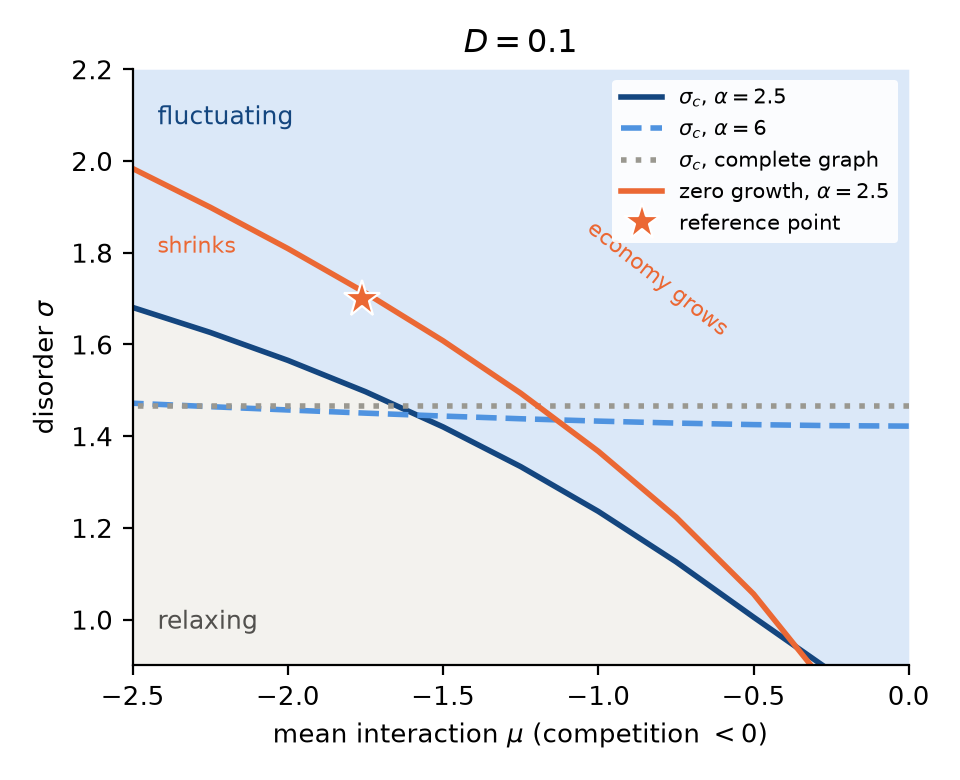
\includegraphics[width=\linewidth]{demographic_phase_diagram.png}
\caption{Phase diagram at $D=0.1$ from the renewal theory.  Above the instability line $\sigma_c(\mu)$ the
composition keeps fluctuating (shaded for the reference graph, $\alpha=2.5$); the lines for $\alpha=6$ and the
complete graph are shown for comparison.  The zero-growth line separates economies whose mean firm
grows from those where it shrinks; above $\sigma_c$ it is the continuation of the static solution and is
not controlled.  The star is the reference point.}
\label{fig:phase}
\end{figure}

%======================================================================
\section{One firm is enough}
\label{sec:onefirm}

Equation~\eqref{eq:onefirm} is exact; its content is that the field can be treated as given, i.e.\
that a firm's own noise does not feed back on its field through the network.  We test this
directly.  We store the fields $\Phi_i(t)$ of two reference economies, integrate
Eq.~\eqref{eq:onefirm} for every node with its measured field and fresh noise, and compare the life
panels.  The exponents agree to $0.011$, the ratios to $0.06$ and the exit rates to $2\%$ for every
minimum life length (SM, Table~S3 and Fig.~S2).  The theory of the
size--volatility statistics is therefore a one-firm problem, given the statistics of the field.


The field follows the degree-resolved law of Eq.~\eqref{eq:hdmft}.  Over the window, a node's mean field
falls with its degree, from $0.5$ at $\kappa\simeq0.4$ to $-2.3$ at $\kappa\simeq2$: hubs compete with more
firms.  Its temporal amplitude grows as $f\propto\kappa^{0.54}$, against $\kappa^{1/2}$ in Eq.~\eqref{eq:hdmft},
and decorrelates over about $4.5$ time units.  Within a degree class the mean field is close to
Gaussian (skewness $-0.3$).  The degree therefore sets both how long a firm lives and how strongly it
is shaken while alive; the second effect drives the multiscaling.

%======================================================================
\section{The volatility law}
\label{sec:law}

\paragraph{Decomposition.}  In logs, Eq.~\eqref{eq:onefirm} reads
$d\ln S=(\Phi-S-D/2S)\,dt+\sqrt{D/S}\,dW$.  Write $\ln S=y_F+\delta$, where $y_F$ solves the noise-free
equation $\dot y_F=\Phi-e^{y_F}$ from the same initial size.  To linear order $\delta$ is an
Ornstein--Uhlenbeck process that relaxes at the local rate $S$ and is driven by noise of variance
$D/S$.  Treating the two parts as independent, the variance of a firm's yearly growth over its life
is
\begin{equation}
\Var g\simeq V_F+B,\qquad B=\Big\langle\frac{D}{S^2}\big(1-e^{-S\Delta t}\big)\Big\rangle_{\rm life},
\label{eq:law}
\end{equation}
where $V_F$ is the growth variance of $y_F$.  The demographic part $B$ tends to $D\Delta t\langle S^{-1}\rangle$
for slowly relaxing firms and to $D\langle S^{-2}\rangle$ for fast ones.

\paragraph{Test.}  For every life with at least $20$ growth rates in the two reference economies we
compute $V_F$ by integrating the noise-free equation along the life's measured field, and $B$ from
its sizes.  Equation~\eqref{eq:law} reproduces the measured volatility to within $5\%$ over a decade and a half of $\Sb$, and $9\%$ in the
lowest decile (Fig.~\ref{fig:law}; SM, Table~S4).  A
version without the filter, $\Var(\Delta\ln\Phi)+D\Delta t\langle S^{-1}\rangle$, overestimates by a nearly constant
factor of $1.5$: a firm does not follow the fast part of its field \todo{scratch result at
$\sigma=1.75$; add to notebooks/04\_volatility\_law.ipynb}.

\begin{figure}[t]
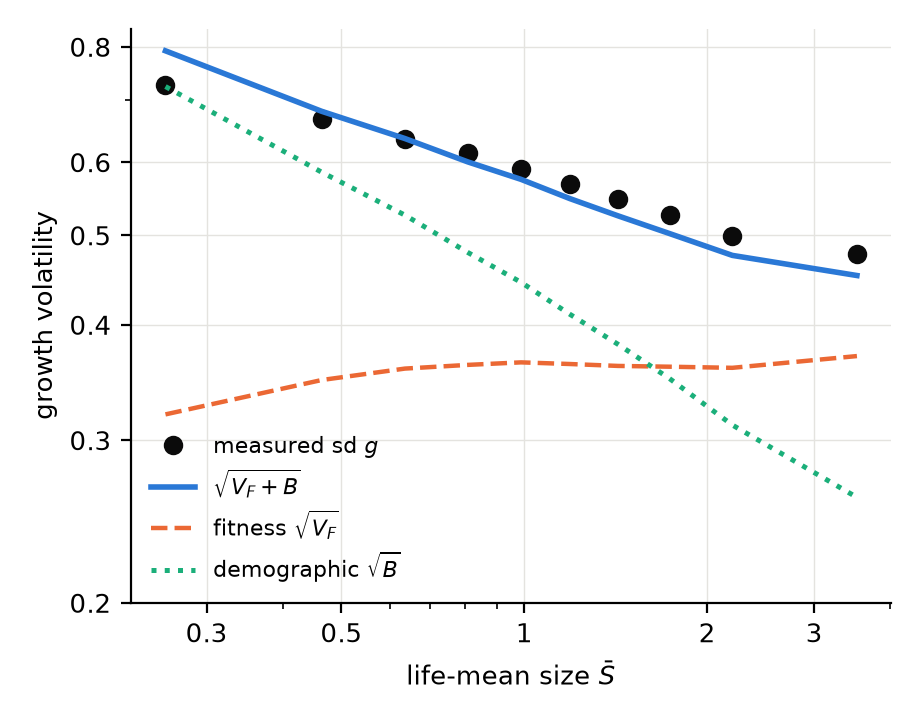
\includegraphics[width=0.85\linewidth]{demographic_volatility_law.png}
\caption{Volatility law, Eq.~\eqref{eq:law}: measured growth volatility, its prediction, and the fitness
and demographic parts, by deciles of life-mean size (lives with at least $20$ growth rates).}
\label{fig:law}
\end{figure}

\paragraph{A crossover.}  The fitness part is nearly flat in size,
$\sqrt{V_F}\simeq0.32$--$0.37$: competition moves established firms by about the same relative
amount whatever their size.  The demographic part falls as $\Sb^{-1/2}$ for small firms and faster for
large ones.  The size--volatility relation is therefore a crossover,
\begin{equation}
v^2\simeq v_F^2+B(\Sb),
\label{eq:crossover}
\end{equation}
from slope $-1/2$, where noise dominates, to slope $0$, where the floor does.  The two parts are equal at
$\Sb\simeq1.5$.  The shape is the one
reported for French firms \cite{fontanelli2025}, and $\zeta_1\simeq0.2$ is the effective slope over the
range where the two parts are comparable.  The crossover scale grows with $D$, so the effective
exponent does too: at $\sigma=1.70$, $\beta=0.20$, $0.21$ and $0.25$ for $D=0.1$, $0.15$ and $0.2$
($n_{\min}=5$; SM, Sec.~S5).

%======================================================================
\section{The multiscaling mechanism}
\label{sec:multiscaling}

\paragraph{An identity.}  Let a firm's squared volatility be the sum of a floor $u_i$ and a part
$B(\Sb)$ common to all firms of the same size, up to an estimation factor $\epsilon_i$ independent of
both: $v_i^2=(u_i+B(\Sb_i))\,\epsilon_i^2$.  Let $b=-d\ln B/d\ln\Sb$ be the local slope of the size-dependent part
and $w=B/(u+B)$ its share of the variance.  Differentiating $\ln\E[v^q\mid\Sb]$ gives
\begin{equation}
\zeta_q=\frac q2\,b\,\langle w\rangle_q,\qquad
\langle w\rangle_q=\frac{\E\big[(u+B)^{q/2}\,w\mid\Sb\big]}{\E\big[(u+B)^{q/2}\mid\Sb\big]},
\label{eq:identity}
\end{equation}
provided the law of $u$ at fixed size does not change with size (the general case adds a composition
term $c_q$; SM, Sec.~S4).  For the demographic part of Eq.~\eqref{eq:crossover} the measured slope is
$b=0.66$--$0.87$ across the range, below the value $1$ of $B\simeq D\Delta t/\Sb$ because $B$ is dominated by
the low excursions of a life.  The exponent is thus about $0.4$ times the noise share, weighted by
$v^q$: largest where noise dominates ($w\to1$) and zero where the floor does ($w\to0$).

\paragraph{When the curve bends.}  Since $\langle w\rangle_q=B\,\E[Y^{q/2-1}]/\E[Y^{q/2}]$ with $Y=u+B$, and
$\ln\E[Y^{q/2}]$ is convex in $q$, $\langle w\rangle_q$ is non-increasing in $q$, and constant only if $Y$ is
the same for all firms of the given size.  Hence
\begin{equation}
\frac{\zeta_q}{\zeta_1}=q\,\frac{\langle w\rangle_q}{\langle w\rangle_1}\le q,
\label{eq:bend}
\end{equation}
with equality if and only if the floor does not vary between firms of equal size.  A floor that is
the same for everybody, however it depends on size, gives a volatility law of fixed shape and
$\zeta_q=q\zeta_1$, like a granular model.  The bend requires heterogeneity of the floor, and it is
strongest where the floor dominates, at large sizes, because there the volatilities of firms with
different floors differ most.  The estimation factor $\epsilon$ cancels in the ratios.  If $\ln Y$ is
Gaussian at fixed size with variance $s^2$, the bend is explicit,
\begin{gather}
\frac{\zeta_q}{\zeta_1}\simeq q\,e^{-(q-1)s^2/2},\nonumber\\
s^2=\Var\big(\ln(u+B)\mid\Sb\big)\simeq(1-w)^2\Var(\ln u\mid\Sb),
\label{eq:lognormal}
\end{gather}
the last form for a narrow floor.  A heterogeneous floor bends the curve only where it is not small
against the demographic part.

\paragraph{The floor on the network.}  The volatility law gives every life its own floor $V_F$, the
growth variance of the noise-free firm along the life's measured field (Sec.~\ref{sec:law}).  For the
lives with at least $20$ growth rates the floor is broad at fixed size, $\Var(\ln V_F\mid\Sb)=0.45$--$0.50$
in the lower three fifths of sizes, rising to $0.85$ in the largest, and the degree explains a growing
share of it, from $14\%$ to $37\%$; overall $V_F\propto\kappa^{0.70}$ (Fig.~\ref{fig:multiscaling}a,b).  The
noise share falls from $\langle w\rangle_1=0.80$ in the smallest fifth to $0.44$ in the largest, and its fall
with $q$ grows with size: $\langle w\rangle_4/\langle w\rangle_1=0.99$, $0.92$, $0.87$, $0.80$, $0.63$
(Fig.~\ref{fig:multiscaling}c).  In the four lower fifths the local exponents of the law agree with
$(q/2)\,b\,\langle w\rangle_q$ to about $10\%$; in the largest the composition term dominates, because the
largest lives also have the largest degrees (mean $\kappa$ $1.01$ in the fourth fifth, $1.51$ in the fifth).

\paragraph{Test.}  We compute the exponents of the same lives under three laws, with the growth
standard deviation as the volatility (Fig.~\ref{fig:multiscaling}d).  Measured, $\zeta_q/\zeta_1=1.77$, $2.35$,
$2.78$.  With each life's own floor and the demographic part replaced by its mean in the life's size
bin, so that the floor is the only source of dispersion, the law predicts $1.86$, $2.57$, $3.10$.  With
the floor replaced instead by its bin mean, the ratios are $2.08$, $3.64$, $6.55$: without the spread of
the floor the curve lies above $q$, because the per-life estimate of the demographic part has its own
dispersion.  The bend of the ratio curve is therefore carried by the heterogeneity of the floor.

\paragraph{Ablation.}  On a random regular graph every firm has degree $C$.  The floor still varies
between lives, $\Var(\ln V_F\mid\Sb)=0.28$--$0.77$, but it is small, and it falls with size, from $0.07$ to
$0.03$ in mean, so that even the largest lives remain dominated by their own noise
($\langle w\rangle_1=0.86$ to $0.69$).  The dispersion of their total variance stays small, $s^2=0.007$ to
$0.05$ from the smallest to the largest fifth, against $0.02$ to $0.25$ on the power-law graph, and the
ratio curve is close to $q$: $1.93$, $2.78$, $3.54$ measured, $1.98$, $2.95$, $3.88$ from the floor alone,
with $\zeta_1=0.40$.  Equation~\eqref{eq:lognormal} with the measured $s^2$ gives $\langle w\rangle_4/\langle w\rangle_1$ to
within $0.06$ in every fifth of both graphs.  On the power-law graph the field amplitude of the larger,
better connected firms keeps their floor at $V_F\simeq0.13$ while their noise falls, and the spread of
degrees spreads the floor: degree heterogeneity is what bends the curve.

\begin{figure*}[t]
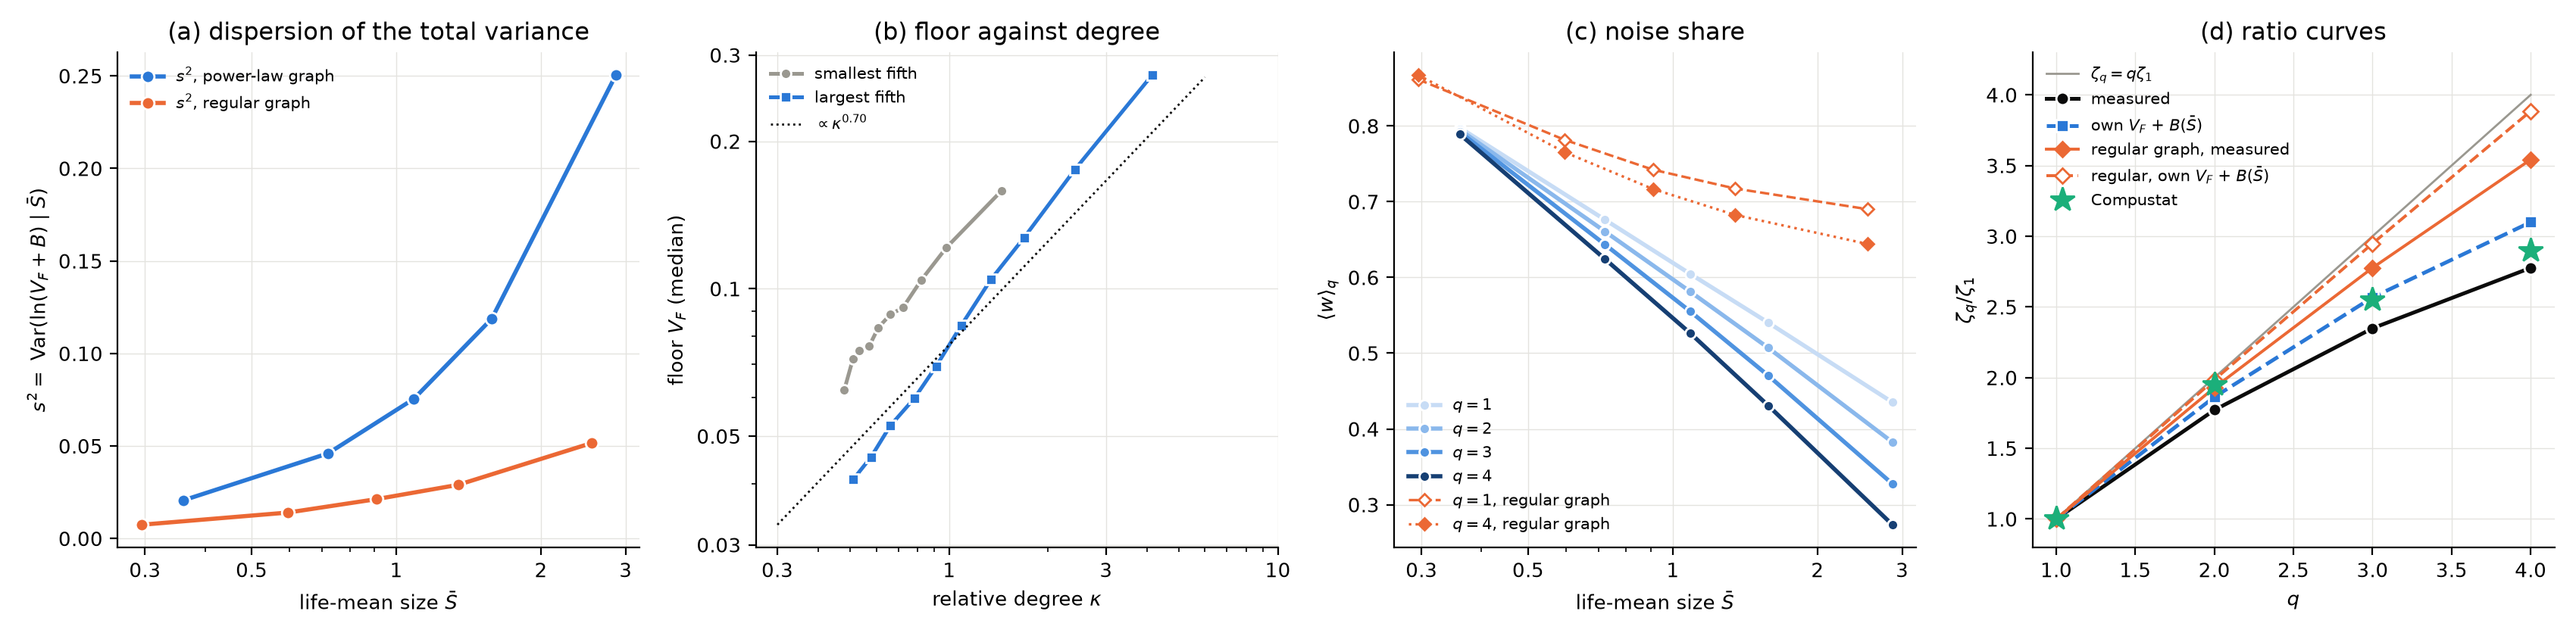
\includegraphics[width=\linewidth]{demographic_multiscaling_law.png}
\caption{Multiscaling mechanism (reference point, $N=16000$, two economies per graph, lives with at
least $20$ growth rates).  (a) Dispersion of the total variance at fixed size,
$s^2=\Var(\ln(V_F+B)\mid\Sb)$ with $B$ at its bin mean, on the power-law and regular graphs.  (b) Median
floor against relative degree in the smallest and largest fifths of sizes (power-law graph).  (c) Noise
share $\langle w\rangle_q$ by size fifth.  (d) Ratio curves: measured, and predicted from each life's floor
plus the bin-mean demographic part, on both graphs; Compustat \cite{moran2024}.}
\label{fig:multiscaling}
\end{figure*}

%======================================================================
\section{Comparison with the firm-growth facts}
\label{sec:facts}

Table~\ref{tab:facts} and Fig.~\ref{fig:facts} compare the reference point with every fact of MSB.

\begin{figure*}[t]
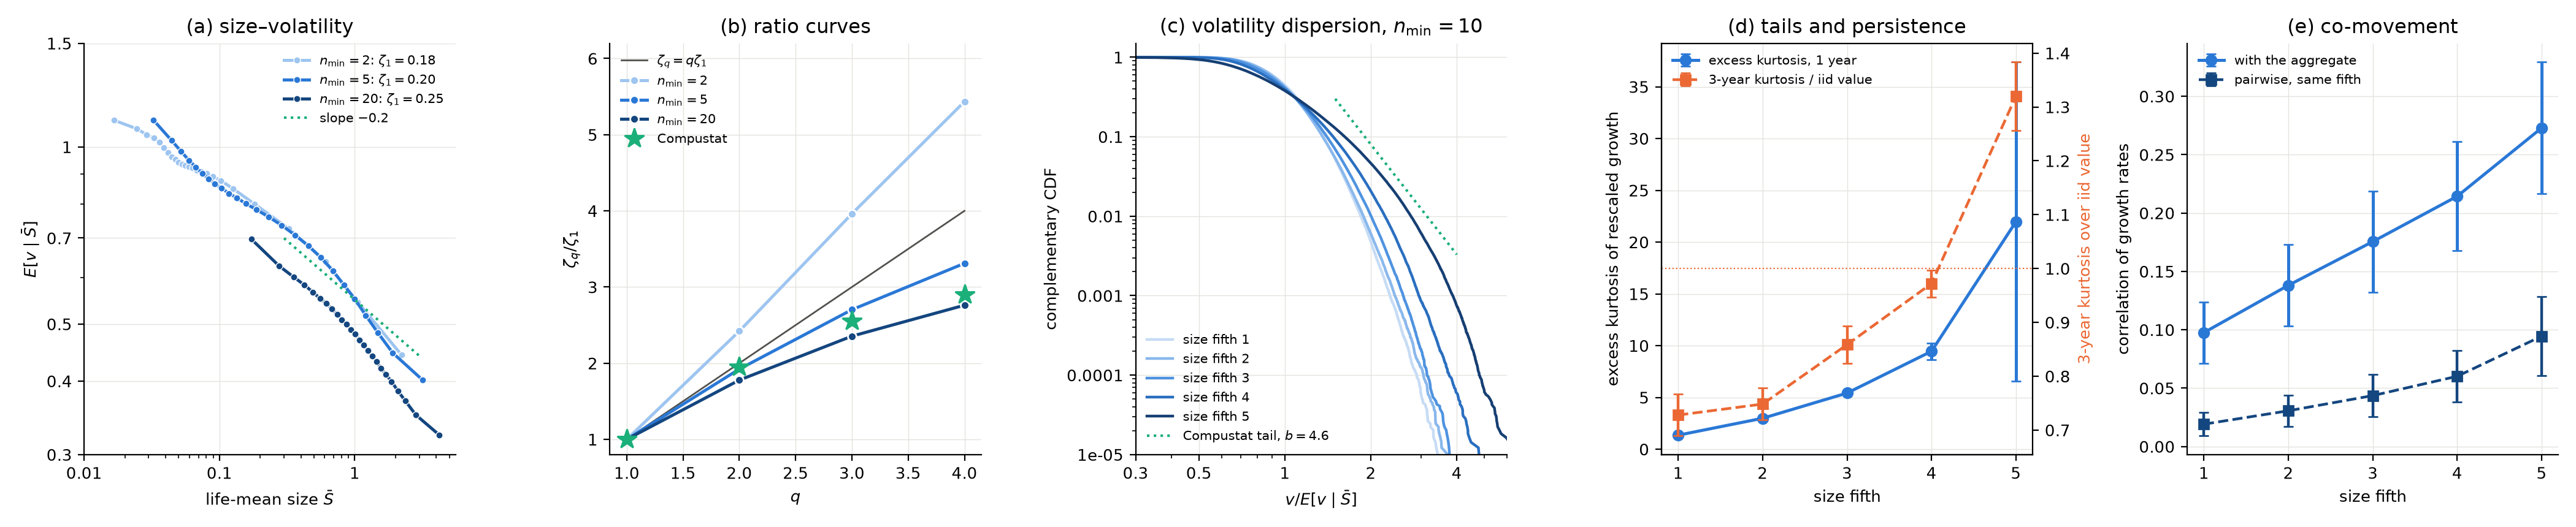
\includegraphics[width=\linewidth]{demographic_prod.png}
\caption{The MSB facts at the reference point ($N=32000$, seven economies pooled, one in a collective
burst excluded; error bars: spread between economies).  (a) Mean volatility against life-mean size for three minimum life lengths.  (b) Ratio
curves against Compustat \cite{moran2024}.  (c) Distribution of $v/\E[v\mid\Sb]$ by fifth of size.  (d) Excess
kurtosis of rescaled yearly growth, and the excess kurtosis of 3-year growth over its iid value, by
size fifth.  (e) Correlation of growth with the aggregate and between firms of the same size fifth.
Source: \texttt{notebooks/06\_facts.ipynb}.}
\label{fig:facts}
\end{figure*}

\begin{table*}[t]
\caption{The MSB facts at the reference point (lives with $n_{\min}=5$ unless stated; $N=32000$, seven
economies) and in Compustat \cite{moran2024}.  Fifths are fifths of
life-mean size.}
\label{tab:facts}
\begin{ruledtabular}
\begin{tabular}{lll}
Fact & Model & Compustat\\
\hline
$\zeta_q$ & $0.21$, $0.39$, $0.55$, $0.68$ & $0.20$, $0.39$, $0.51$, $0.58$\\
$\zeta_1$, spread between economies & $\pm0.02$ & \\
$\zeta_q/\zeta_1$ & $1.92$, $2.70$, $3.31$ & $2.0$, $2.6$, $2.9$\\
$\zeta_q/\zeta_1$, $n_{\min}=20$ & $1.78$, $2.35$, $2.76$ & \\
$\zeta_q/\zeta_1$, $n_{\min}=2$ & $2.42$, $3.96$, $5.43$ & $2.0$, $2.6$, $2.9$\\
range of the decline & $2.0$ decades & $4$ decades\\
volatility, smallest $\to$ largest bin & $1.11\to0.40$ & $1.22\to0.22$\\
hump at small sizes & none & none\\
tail $b$ of $v/\E[v\mid\Sb]$, $n_{\min}=10$ & $5.5$ & $4.6$\\
excess kurtosis of rescaled growth & $1.4\to22$ by fifth & roughly constant\\
3-year persistence (kurtosis/iid) & $0.73\to1.32$ by fifth & $>1$ at all sizes\\
correlation with the aggregate & $0.10\to0.27$ by fifth & rises with size\\
pairwise correlation, same fifth & $0.02\to0.09$ & rises with size\\
size distribution & Hill index $4.5$ & Zipf, $\simeq1$\\
\end{tabular}
\end{ruledtabular}
\end{table*}

\paragraph{What the model explains.}  The disorder $\sigma$ and the noise $D$ were chosen so that
$\zeta_1\simeq0.2$; everything else follows.  The life panel declines monotonically, with no hump at small sizes, with $\zeta_q$ close to
the Compustat values for $q\le3$ and a ratio curve that bends below $q$: by less than in Compustat for
lives with $n_{\min}=5$ ($3.31$ against $2.9$ at $q=4$), and by about the empirical amount for $n_{\min}=20$
($1.78$, $2.35$, $2.76$).
The bend comes from the mechanism of Sec.~\ref{sec:multiscaling}.  The co-movement of a firm with the
aggregate and with firms of similar size rises with size, as in Compustat; a natural reading is that
small firms are moved mostly by their own noise and large ones by their field, which they share with
their neighbours, but we have no theory of it.  The shape of the curve, $\zeta_q$ and the ratios survive
$N=8000$--$64000$, different seeds and the neighbourhood of the reference point in $\sigma$, $D$, $\alpha$
and $C$; $\sigma$, $D$ and $C$ set the level of $\zeta_1$ (SM, Sec.~S5).

\paragraph{What it does not.}
\begin{itemize}
\item \emph{Short lives.}  With MSB's baseline sample, lives with at least two growth rates, the
  ratios lie above $q$: very short lives are newborns dominated by their own noise, whose
  volatility estimates are dispersed most among the smallest firms.  Only lives with $n_{\min}\gtrsim5$
  show the bend.
\item \emph{Large firms are too volatile and too fat-tailed.}  Volatility falls by a factor $2.8$
  over two decades against $5.5$ over four in Compustat.  The rescaled growth rates of small firms
  are nearly Gaussian and those of large firms strongly fat-tailed, and multi-year persistence is
  confined to the largest firms.  Small firms are moved by near-Gaussian, mean-reverting birth--death
  noise, large firms by rare and persistent dips of their field.
\item \emph{The tail of the volatility distribution.}  At $n_{\min}=10$ the model gives $b\simeq5.5$
  against $4.6$.  The model's $b=4.4$ at $n_{\min}=2$ is an artefact of short lives: a null with iid
  Laplace growth and no differences between firms gives $4.3$ (SM, Sec.~S6).
\item \emph{Aggregate volatility} is several times too large and does not fall as $N^{-1/2}$ over the
  sizes we simulate.  Occasionally an economy enters a collective burst, with aggregate volatility
  several times the typical one, in which volatility no longer depends on size (about $5$ of $90$
  economies across all our runs; SM, Sec.~S5).
\item \emph{Sizes and demography.}  The size distribution has no Pareto tail, newborns have extreme
  infant mortality, and small established firms shrink on average.
\end{itemize}

%======================================================================
\section{Why the range is short and there is no Zipf law}
\label{sec:limits}

The self-limitation $-x_i/m$ in Eq.~\eqref{eq:model} does two jobs.  It bounds a firm whose field stays
favourable, which keeps the economy from condensing onto the best niche, and its restoring rate is
what makes volatility depend on size: the demographic part of Eq.~\eqref{eq:law} is filtered at the
rate $S$, and the floor is set by how a firm on its plateau $x=m\Phi$ follows its field.  Both rely on the
plateau, and the plateau caps firms at a few times the mean.  The decline therefore runs from a few
times the newborn size $D$, below which lives are too short to measure, to the plateau: about two
decades at the reference point.

\paragraph{The exponent and the range trade off.}  Replace the self-limitation and the interactions by
powers, $(x_i/m)^\theta$ and $\sum_jJ_{ij}(x_j/m)^\theta$.  Without noise, $u_i=S_i^\theta$ obeys the
$\theta=1$ model with time rescaled by $\theta$, and since $\ln S=\theta^{-1}\ln u$,
\begin{equation}
\beta_S=\theta\,\beta_u,\qquad R_S=R_u/\theta,
\label{eq:product}
\end{equation}
with $R$ the number of decades over which volatility declines.  A softer self-limitation widens the
range by exactly the factor by which it flattens the decline, and the product $\beta R$ is fixed by the
statistics of the field: about $0.3$--$0.4$ in the model against $0.8$ in Compustat \todo{check with the
noise term, which breaks the exact mapping below the noise crossover}.  Keeping the interactions
linear while softening only the self-limitation condenses the economy.

\paragraph{Other ways out.}  Without self-limitation, growth is Gibrat-like, the condition under which a
lower barrier gives Zipf's law \cite{gabaix1999}, but the quenched part of the field is not removed and
the economy condenses onto the best niche.  Giving each firm its own scale, a capacity $K_i$ that
moves in time, keeps the plateau but makes volatility depend only on $S_i/K_i$, so a Zipf law of
capacities comes with $\zeta_1=0$; making competitors act through their absolute sizes lets the largest
firms dominate every field.  A model with both a Zipf law and a volatility law over four decades
needs a size dependence of the dynamics that is not tied to a plateau, which in a one-variable model
means an explicit exponent.  We read this as a limit of self-limited growth rather than of the
particular model.

%======================================================================
\section{Discussion}
\label{sec:discussion}

An economy of firms that compete on a heterogeneous network and are subject to birth--death noise
reproduces the shape of the size--volatility relation of firms: a monotone decline with effective
exponent $0.2$ and a ratio curve $\zeta_q/\zeta_1$ that bends below $q$.  The theory is a one-firm problem:
a logistic unit driven by a Gaussian field whose amplitude grows as the square root of its degree,
plus its own noise.  The exponent is the effective slope of a crossover between a demographic regime
of slope $-1/2$ and a fitness floor of slope $0$, which is the two-regime shape of data that include
small firms \cite{fontanelli2025}.  The multiscaling has a simple origin: a volatility law of the form
floor plus size-dependent part gives $\zeta_q=(q/2)b\langle w\rangle_q$, and the curve bends below $q$ exactly
when the floor differs between firms of equal size.  Granular models give a fixed shape and ratios
$q$; heterogeneous interactions give a heterogeneous floor and the bend.

The identity~\eqref{eq:identity} does not depend on the network model, and suggests two tests on
firm data.  First, the dispersion of volatilities among firms of equal size should grow with size,
and a measure of a firm's exposure to others---its number of customers, suppliers or competitors---
should explain a growing share of it.  Second, conditioning on that exposure should move the ratio
curve towards $q$.  The model also predicts that the decline steepens towards slope $-1/2$ for the
smallest firms, below the sizes covered by Compustat.

The model fails where the self-limitation it relies on bites: the range of the decline is two decades
rather than four, sizes have no Pareto tail, and large firms are too volatile.  Section~\ref{sec:limits}
shows that these failures are tied together.  Open problems are a two-time theory with noise and
turnover, which would give the field's correlation above $\sigma_c(D)$ and with it the floor $v_F$ and
$\zeta_1(\sigma,D)$ without simulation; the rising co-movement with size, which involves the common mode
of a finite economy; and a dynamics that decouples the volatility decline from the size cap.

\bibliography{bib}

\end{document}
